\subsubsection{Gestão de avaliações}

A página de avaliações contém um resumo das avaliações à que um aluno foi sujeito. Esta apresenta as unidades curriculares em que o aluno está inscrito, organizada pelo ano letivo destas. Apenas são mostradas unidades curriculares que contêm projetos.

Em cada unidade curricular é feita uma referência ao curso a que esta se refere e é listado os projetos desta.

Para cada projeto, além da respetiva nota, também são listadas as fases deste e respetiva nota.

Na Figura~\ref{fig:student_grades} pode ser consultada uma imagem demonstrativa da página desenvolvida.

\begin{figure}[H]
  \centering
  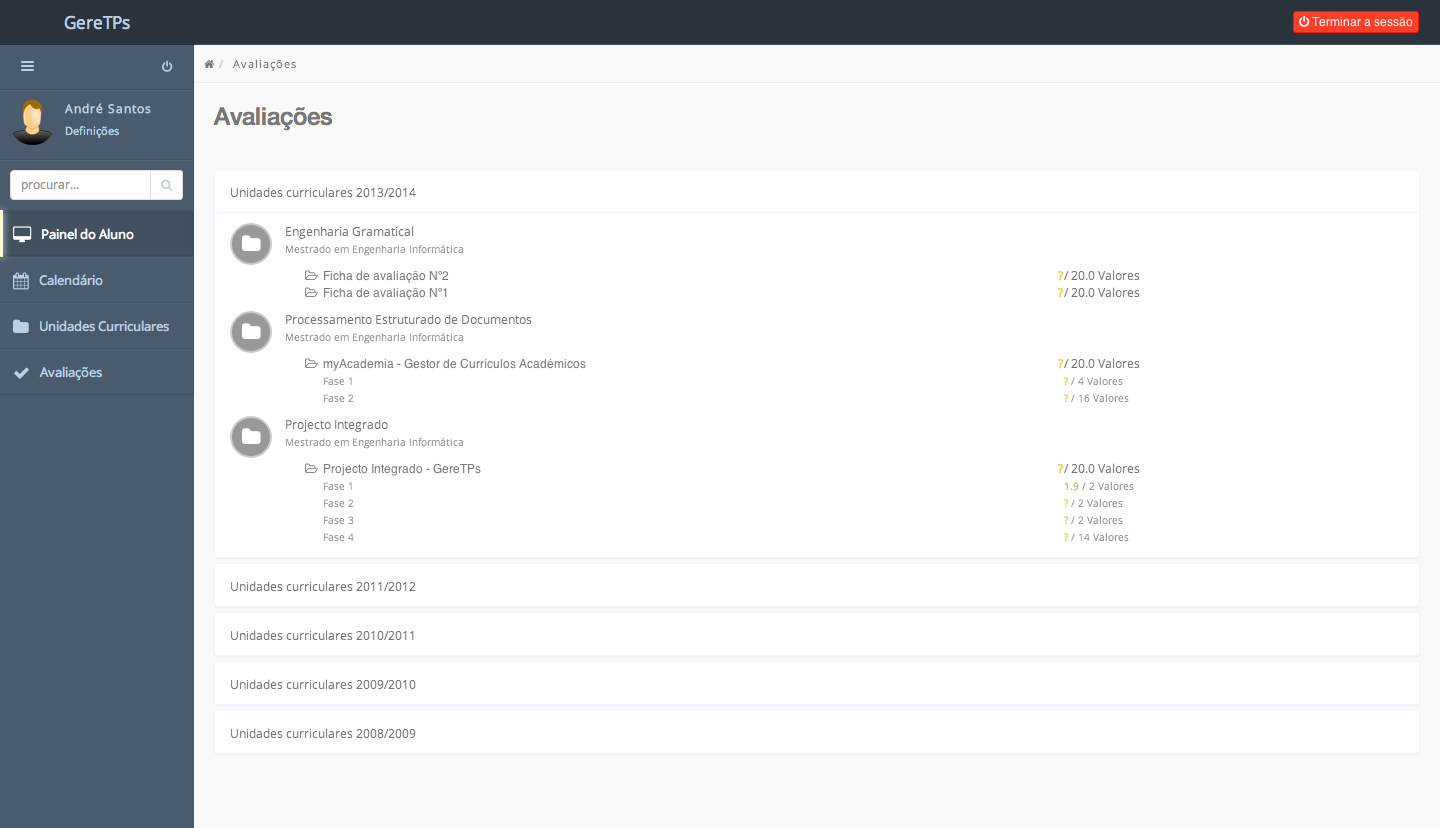
\includegraphics[width=1\textwidth,center]{images/implementacao/alunos/grades}
  \caption{Avaliações de um aluno}
  \label{fig:student_grades}
\end{figure}
